\section{Fuzzy system}
%Introduzione
\subsection{Introduzione}
\uline{La logica fuzzy è un approccio al calcolo basato sul "grado di verità" anziché sulla solita logica booleana vera o falsa ($1$ o $0$) con risposte a mutua esclusione}

La logica classica si basa su una visione binaria del mondo, dove ogni proposizione può essere vera o falsa. Molte proposizioni sul mondo reale non sono né vere né false. Questa visione può essere inadeguata quando si tratta di modellare concetti complessi, che non hanno definizioni precise e possono presentare sfumature e \textit{gradi di verità} diversi. In questi casi, la logica fuzzy e la teoria degli insiemi fuzzy possono essere utilizzate per rappresentare e ragionare. È importante notare che l'imprecisione non deve essere confusa con l'incertezza, che si riferisce alla possibilità che un evento si verifichi o meno espressa attraverso la probabilità. \uline{La probabilità rimane un fenomeno booleano, mentre l'appartenenza fuzzy si riferisce a quanto un oggetto soddisfa una determinata proprietà}.

\paragraph{Esempio}
Ad esempio, una persona non avrà problemi ad accelerare lentamente mentre avvia una macchina, se gli viene chiesto di farlo. Se vogliamo automatizzare questa azione, non sarà affatto chiaro come tradurre questo consiglio in un'azione di controllo ben definita. È necessario determinare una dichiarazione concreta basata su un valore non ambiguo, ad esempio "premi l'acceleratore alla velocità di mezzo centimetro al secondo". D'altra parte, questo tipo di informazione non sarà adeguata o molto utile per una persona. In questo caso, un problema principale sarà la traduzione della descrizione verbale in valori concreti, ad esempio assegnando "premi l'acceleratore lentamente" a "premi l'acceleratore alla velocità di un centimetro al secondo".

\paragraph{Fuzzy set}
A differenza degli insiemi tradizionali, in cui un elemento può o non può appartenere all'insieme, in un insieme fuzzy ogni elemento ha un grado di appartenenza compreso tra $0$ e $1$. Questo grado di appartenenza rappresenta il livello di membership o la probabilità di appartenenza dell'elemento all'insieme

\begin{definizione}
Dato un dominio del discorso $X$, un insieme fuzzy $\mu$ è una funzione $\mu : X \to [0,1]$ che assegna ad ogni elemento un grado di appartenenza $\mu(x)$ rispetto all'insieme $\mu$.
\end{definizione}

\uline{I fuzzy set rappresentano un'interfaccia tra il linguaggio naturale e le sue corrispondenti rappresentazioni numeriche}. E' possibile associare un valore numerico ad un'espressione linguistica che descrive un concetto sfumato o non preciso, in modo da poter utilizzare tali valori per l'analisi e la manipolazione dei dati.

Ad esempio, vogliamo dare un modello formale alla proprietà "essere alto per un bambino di $4$ anni". Per farlo definiremo un insieme fuzzy $\mu_{tall}$ attraverso una funzione sigmoide come in figura, tale per cui risulteranno sicuramente nell’estensione della proprietà i bambini più alti di $1.5m$ centimetri e sicuramente fuori dall’estensione quelli più bassi di $0.7m$. Tutti gli altri apparterranno all’insieme con un certo grado.

\begin{figure}[h]
    \centering
    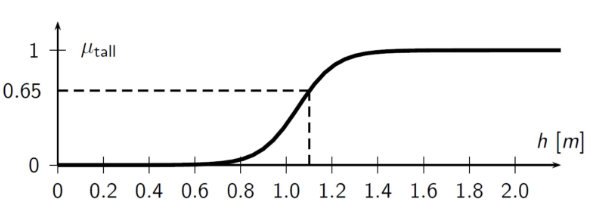
\includegraphics[scale=0.4]{images/utall.png}
    \caption{L’insieme fuzzy $\mu_{tall}$ che descrive il predicato "essere alto per un bambino di $4$ anni"}
\end{figure}

\paragraph{Semantiche della funzione di appartenenza}
Esistono diverse interpretazioni possibili per la funzione di appartenenza fuzzy, a seconda dell'applicazione in cui viene utilizzata. In particolare
\begin{enumerate}
    \item \textit{Somiglianza}, la funzione di appartenenza viene interpretata come il \textit{grado di prossimità} di un elemento rispetto ad un prototipo, e viene utilizzata in problemi di classification, clustering e regression
    \item \textit{Preferenza}, negli insiemi fuzzy, la preferenza viene rappresentata attraverso la funzione di appartenenza, che indica il grado di soddisfazione o di preferenza per un determinato oggetto o un dato valore. La funzione di appartenenza viene interpretata come l'intensità della preferenza associata all'oggetto. Più il grado di appartenenza di un oggetto a un insieme fuzzy è elevato, maggiore sarà l'intensità della preferenza per quell'oggetto. Il grado di appartenenza, nell'ambito della preferenza, fornisce un modo per quantificare e misurare l'intensità o la forza della preferenza per gli oggetti o le decisioni prese
    \item \textit{Possibilità}, la funzione di appartenenza viene interpretata come il \textit{grado di possibilità} che un elemento sia il valore di un parametro $X$. Questa interpretazione viene utilizzata per quantificare lo stato epistemico di un agente, distinguendo ciò che è "sorprendente" da ciò che è "tipico" o "aspettato"
\end{enumerate}

\paragraph{Funzioni triangolari e trapezoidali}
Di solito gli insiemi fuzzy vengono utilizzati per modellare espressioni, a volte chiamate anche espressioni linguistiche, al fine di sottolineare la relazione con il linguaggio naturale, ad esempio "circa 3", "di altezza media" o "molto alto", che descrivono un valore impreciso o un intervallo impreciso. Gli insiemi fuzzy associati a tali espressioni dovrebbero aumentare in modo monotono fino a un certo valore e diminuire in modo monotono da tale valore. Tali insiemi fuzzy sono chiamati \textit{convessi}. Le funzioni che rappresentano insiemi convessi sono dette \textit{funzioni triangolari}, rappresentate come
$$
\Lambda_{a,b,c} : \mathbb{R} \to [0,1],\quad x \mapsto 
    \begin{cases}
        \frac{x-a}{b-a} \text{ if } a \leq x < b \\
        \frac{c-x}{c-b} \text{ if } b \leq x \leq c \\
        0 \quad \text{  altrimenti}
    \end{cases}
$$

Le funzioni triangolari possono essere considerate un caso particolare delle \textit{funzioni trapezoidali}
$$
\Pi_{a,b,c,d} : \mathbb{R} \to [0,1],\quad x \mapsto 
    \begin{cases}
        \frac{x-a}{b-a} \text{ if } a \leq x \leq b \\
        1 \quad \text{ if  }  b \leq x \leq c \\
        \frac{d-x}{d-c} \text{ if } c \leq x \leq d \\
        0 \quad \text{  altrimenti}
    \end{cases}
$$

 \begin{definizione}
Sia $\mu$ un fuzzy set definito rispetto al dominio del discorso $X$ e sia $\alpha \in [0,1]$. L'insieme
$$[\mu]_\alpha = \{x \in X \;|\; \mu(x) \geq \alpha \}$$
è chiamato $\alpha$-cut o $\alpha$ level set dell'insieme $\mu$.
 \end{definizione}

\paragraph{Vertical view}
La rappresentazione di un insieme fuzzy come una funzione dall'universo del discorso all'intervallo unitario, che assegna un grado di appartenenza a ciascun elemento, viene chiamata visione verticale. Il fuzzy set può essere visto come un inviluppo superiore dei suoi alpha cut

\paragraph{Horizontal view}
Un'altra possibilità per descrivere un insieme fuzzy è la visione orizzontale. Per ogni valore $\alpha$ dell'intervallo unitario, consideriamo l'insieme degli elementi che hanno un grado di appartenenza almeno $\alpha$ all'insieme fuzzy

Gli insiemi di livello di un insieme fuzzy hanno l'importante proprietà di caratterizzare univocamente l'insieme fuzzy stesso. Quando conosciamo gli insiemi di livello $[\mu]\alpha$ di un insieme fuzzy $\mu$ per tutti gli $\alpha \in [0, 1]$, possiamo determinare il grado di appartenenza $\mu(x)$ di qualsiasi elemento $x$ a $\mu$ tramite l'equazione
$$\mu(x) = \sup_{\alpha \in [0,1]} \{x \in [\mu]_{\alpha}\}$$

%Definizioni alpha-cut
\subsubsection{Definizioni alpha-cut}
Avendo introdotto gli alpha-cut come uno strumento per rappresentare i fuzzy set, ora li sfrutteremo definendo alcuni concetti molto utili

\paragraph{Supporto}
Il supporto $S(\mu)$ di un insieme fuzzy $\mu$ è l'insieme booleano che contiene tutti e soli gli elementi del dominio del discorso che hanno un grado di appartenenza non nullo rispetto a $\mu$. Tutti gli elementi del dominio
$$S(\mu) = [\mu]_{\bar{0}} = \{ x \in X | \mu(x) > 0 \}$$

\paragraph{Centro}
Il centro $C(\mu)$ di un insieme fuzzy $\mu$ è l'insieme booleano che contiene tutti e soli gli elementi del dominio del discorso che hanno un grado di appartenenza uguale a 1 rispetto a $\mu$
$$C(\mu) = [\mu]_{1} = \{ x \in X | \mu(x) = 1 \}$$

\paragraph{Altezza}
L'altezza $h(\mu)$ di un insieme fuzzy $\mu$ è il più alto grado di appartenenza ottenibile da un elemento di $\mu$
$$h(\mu) = \sup_{x \in X} \{\mu(x)\}$$
Un insieme fuzzy $\mu$ è definito normale sse $h(\mu) = 1$, altrimenti sub-normale

\paragraph{Convesso}
Un insieme fuzzy $\mu$ è definito convesso\footnote{Un insieme convesso è un insieme in cui, presi due punti qualsiasi all'interno dell'insieme, la linea che li congiunge è completamente contenuta all'interno dell'insieme stesso. In altre parole, tutti i punti sulla linea che collega due punti dell'insieme sono anch'essi contenuti nell'insieme} sse i suoi alpha-cut/level set sono convessi per ogni scelta di $\alpha \in [0,1)$

\paragraph{Numero fuzzy}
Un insieme fuzzy $\mu$ è un numero fuzzy sse $\mu$ è normale e $[\mu]\alpha$
è chiusa, limitata e convessa per ogni scelta di $\alpha \in [0,1)$. Va a generalizzare l'aritmetica che si fa con i numeri reali

%Logica fuzzy
\subsection{Logica fuzzy}
La logica classica e la teoria degli insiemi finiti sono equivalenti e possono essere rappresentate tramite un'algebra booleana finita. Gli operatori logici di congiunzione, disgiunzione e negazione possono essere utilizzati per definire gli operatori insiemistici. Nella logica fuzzy, l'intervallo reale $[0,1]$ rappresenta l'insieme dei valori di verità e gli operatori logici booleani vengono adattati per aderire alla nuova semantica. Quindi, è possibile costruire una teoria degli operatori insiemistici "fuzzy" utilizzando gli stessi operatori logici della logica classica.

I connettivi logici più importanti sono il logico AND $\land$ (congiunzione), il logico OR $\lor$ (disgiunzione), la negazione NOT $\lnot$ e l'IMPLICAZIONE $\rightarrow$. Le funzioni di verità più comunemente usate per la congiunzione e la disgiunzione nella logica fuzzy sono il minimo o il massimo. Ciò significa che

\begin{enumerate}
\item{$\neg \mu \doteq 1 - \mu(x)$} 
\item{$\mu \wedge \mu' \doteq \min\{\mu(x),\mu'(x)\}$}
\item{$\mu \vee \mu' \doteq \max\{\mu(x),\mu'(x)\}$}
\end{enumerate}

\paragraph{Negazione stretta e forte}
Esistono vari modi di definire la negazione in una logica fuzzy. L’unico requisito è che la definizione rispetti tre proprietà che, intuitivamente, ogni negazione deve possedere:
\begin{enumerate}
    \item{$\neg(0) = 1$} 
    \item{$\neg(1) = 0$}
    \item{$x \leq y \implies \neg x \geq \neg y$}
\end{enumerate}

In aggiunta a queste proprietà, una negazione può soddisfarne altre. Per esempio, si può chiedere che sia \textit{strettamente decrescente}
$$x < y \implies \neg x > \neg y$$
Che sia \textit{continua}, se soddisfa la proprietà di continuità, che afferma che piccole variazioni nei valori di verità delle proposizioni corrispondono a piccole variazioni nei valori di verità delle loro negazioni. In altre parole, se due proposizioni fuzzy sono molto simili, le loro negazioni dovrebbero essere anche molto simili.

O \textit{involutiva}:
$$\neg \neg x = x$$

\begin{definizione}
    Una negazione si dice stretta sse è strettamente decrescente e
    continua
\end{definizione}

\begin{definizione}
    Una negazione si dice forte sse è stretta e involutiva
\end{definizione}

\paragraph{T-norme e t-conorme}
Le t-norme (triangular norms) e le t-conorme (triangular conorms) sono utilizzate nella logica fuzzy per definire le operazioni di congiunzione e disgiunzione tra le proposizioni fuzzy.

Le t-norme sono funzioni che prendono in input due valori di verità (compresi tra 0 e 1) e restituiscono un valore di verità che rappresenta la congiunzione delle due proposizioni fuzzy. Una funzione $\top : [0,1]^2 \to [0,1]$ si dice \textit{t-norma} sse soddisfa le seguenti proprietà:
\begin{enumerate}
    \item Commutativa: {$\top(x,y) = \top(y,x)$}
    \item Associativa: {$\top(x,\top(y,z)) = \top(\top(x,y),z)$}
    \item Monotonicità: {$x \leq z \implies \top(x,y) \leq \top(x,z)$}\\
    cioè il valore di verità della congiunzione $x \land z$ non dovrebbe essere inferiore al valore di verità della congiunzione $x \land y$, se $x$ ha un valore di verità inferiore a $z$.
    \item Identità: {$\top(x,1) = x$}\\
    richiediamo che il valore di verità di una proposizione $x$ sia lo stesso del valore di verità della congiunzione di $x$ con qualsiasi proposizione vera $y$.
\end{enumerate}
Nel contesto della logica fuzzy, è conveniente utilizzare una t-norma come funzione di verità per la congiunzione. La proprietà $4$ implica che per ogni t-norma $t$, abbiamo $t(1, 1) = 1$ e $t(0, 1) = 0$. Inoltre, grazie alla proprietà $1$, otteniamo $t(1, 0) = 0$ a partire da $t(0, 1) = 0$. Infine, grazie alla proprietà di monotonicità $3$ e $t(0, 1) = 0$, otteniamo $t(0, 0) = 0$. Pertanto, ogni t-norma, quando limitata ai valori $0$ e $1$, coincide con la funzione di verità della congiunzione usuale data dalla tabella di verità.

Le t-conorme sono funzioni che prendono in input due valori di verità e restituiscono un valore di verità che rappresenta la disgiunzione delle due proposizioni fuzzy. Una funzione $\bot: [0,1]^2 \to [0,1]$ si dice \textit{t-conorma} sse soddisfa le seguenti proprietà:
\begin{enumerate}
    \item Commutativa: {$\bot(x,y) = \bot(y,x)$}
    \item Associativa: {$\bot(x,\bot(y,z)) = \bot(\bot(x,y),z)$}
    \item Monotonicità: {$x \leq z \implies \bot(x,y) \leq \bot(x,z)$}
    \item Identità: {$\bot(x,0) = x$}\\
    ciò significa che il valore di verità di una proposizione $x$ sarà lo stesso del valore di verità della disgiunzione di $y$ con una proposizione falsa $x$
\end{enumerate}

\paragraph{Implicazione fuzzy}
Nell'ambito della logica fuzzy, le regole fuzzi sono state usate per definire come le variabili di input influenzano quelle di output. Ogni regola è composta da due parti: l'antecedente (if) e il conseguente (then). Le implicazioni sono operatori matematici che collegano l'antecedente al conseguente.

Come nel caso booleano avremo che un insieme fuzzy è contenuto in un altro se tutti gli elementi del primo sono contenuti nel secondo. Sfruttando l’isomorfismo tra operatori logici e insiemistici, inoltre potremo definire il concetto di sottoinsieme a partire da quello di implicazione come segue
$$I(a,b) = \neg a \vee b$$
A seconda della semantica che daremo ai nostri operatori logici fuzzy avremo varie classi di implicazioni:
\begin{enumerate}
    \item{\textit{S-implication}: $I(a,b) = \bot(\neg a, b)$}
    \item{\textit{Residuated implication}: $I(a,b) = \sup \{x \in [0,1] | \top(a,x) \leq b\}$}, basato sul concetto di residuo nella teoria delle reti di Kleene
    \item{\textit{Quantum Logic-implication}: $I(a,b) = \bot(\neg a, \top(a,b))$}, meccanica quantistica
\end{enumerate}

\paragraph{Linguistic Modifiers}
Normalmente, un fuzzy set rappresenta un concetto impreciso come "velocità elevata", "giovane" o "alto". Da tali concetti possiamo derivare altri concetti imprecisi applicando dei modificatori linguistici (linguistic hedges) come "molto" o "più o meno".

Una velocità molto alta è anche una velocità elevata, ma non viceversa. Pertanto, il grado di appartenenza di una specifica velocità $v$ al fuzzy set $\mu_{vhv}$ non dovrebbe superare il suo grado di appartenenza al fuzzy set $\mu_{hv}$. Possiamo ottenere ciò interpretando il modificatore linguistico "molto", simile alla negazione, come un operatore unario e assegnando una funzione di verità adeguata ad esso, ad esempio $w_{very(\alpha)} = \alpha^2$. In questo modo otteniamo $\mu_{vhv(x)} = (\mu_{hv(x)})^2$. Ora, una velocità che è in misura di $1$ una velocità elevata è anche una velocità molto alta. Una velocità che non è una velocità elevata (grado di appartenenza $0$) non è nemmeno una velocità molto alta. Se il grado di appartenenza di una velocità a $\mu_{hv}$ è compreso tra $0$ e $1$, essa è anche una velocità molto alta, ma con un grado di appartenenza inferiore.

Nello stesso modo possiamo assegnare una funzione di verità al modificatore "più o meno". Questa funzione di verità dovrebbe aumentare il grado di appartenenza, ad esempio $w_{more or less(\alpha)} = \sqrt{\alpha}$.


\begin{figure}[h]
    \centering
    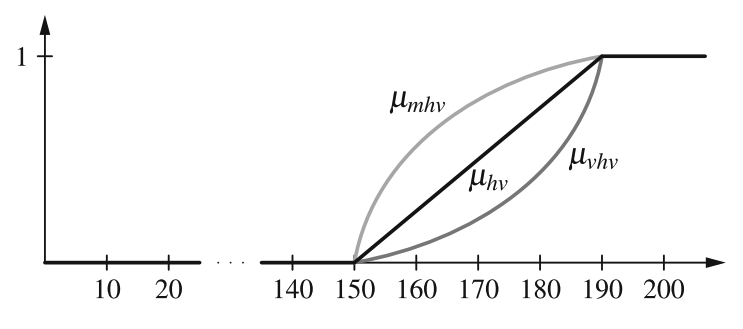
\includegraphics[scale=0.4]{images/linguistic-modifiers.png}
    \caption{I fuzzy set $\mu_{hv}$, $\mu_{vhv}$ e $\mu_{mhv}$ di velocità elevate, molto elevate e più o meno elevate}
\end{figure}
%Teoria
\subsection{Teoria della logica fuzzy}

\paragraph{Principio di estensione}
Permette di generalizzare una qualsiasi funzione $G$ da insiemi classici ad insiemi fuzzy

Un insieme fuzzy è caratterizzato da gradi di appartenenza, che indicano in che misura gli elementi dell'universo del discorso appartengono all'insieme fuzzy. \uline{Il principio di estensione ci fornisce una regola per calcolare il grado di verità degli elementi dell'insieme immagine basandoci sui gradi di verità degli elementi originali dell'insieme fuzzy}

Il principio di estensione si basa sull'idea fondamentale di associare a ciascun elemento dell'insieme immagine un grado di appartenenza che rappresenta la massima appartenenza possibile tra tutti gli elementi dell'insieme di partenza che vengono mappati su quell'elemento specifico

In altre parole, il principio di estensione stabilisce che il grado di appartenenza di un elemento all'immagine\footnote{L'immagine di un insieme attraverso una funzione è un concetto che descrive l'insieme dei valori che la funzione assume quando viene applicata agli elementi dell'insieme di partenza. Più precisamente, data una funzione $f: X \rightarrow Y$, dove $X$ è l'insieme di partenza e $Y$ è l'insieme di arrivo, l'immagine di un insieme $A \subseteq X$, indicata come $f[A]$, è l'insieme dei valori che la funzione $f$ assume quando viene applicata agli elementi di $A$. In altre parole, $f[A] = {y \in Y | \exists x \in A : f(x) = y}$. Può aiutarci a studiare la relazione tra gli elementi di due insiemi e a identificare proprietà importanti della funzione stessa} di un insieme fuzzy è determinato dalla massima appartenenza tra tutti gli elementi dell'insieme di partenza che sono mappati su quell'elemento specifico dell'insieme di arrivo. Il principio di estensione, nel contesto degli insiemi fuzzy, ci consente di estendere il concetto di immagine anche agli insiemi fuzzy.

\paragraph{Alcuni insiemi fuzzy rilevanti}
Esistono diversi tipi di insiemi fuzzy, ma quelli definiti sull'insieme dei numeri reali sono particolarmente importanti perché hanno un significato quantitativo che può essere utilizzato per rappresentare variabili fuzzy. Queste variabili sono fondamentali in molte applicazioni come il controllo fuzzy, il ragionamento approssimato e l'ottimizzazione. In letteratura, ci sono alcune classi di $F(\mathbb{R})$, l'insieme degli insiemi fuzzy sui reali, che sono spesso citate, tra cui:
\begin{enumerate}
    \item{Normal fuzzy set: \\ $F_N(\mathbb{R}) = \{\mu \in F(\mathbb{R}) | \exists x \in \mathbb{R} : \mu(x) = 1 \}$}
    \item{Upper Semi-continuous fuzzy set: \\$F_C(\mathbb{R}) = \{\mu \in F_N(\mathbb{R}) | \forall \alpha \in (0,1] : [\mu]_\alpha \text{ è compatto }\}$}
    \item{Fuzzy interval: \\ $F_I(\mathbb{R}) = \{\mu \in F_N(\mathbb{R}) | \forall a,b,c \in \mathbb{R} : c \in [a,b] \implies \mu(c) \geq \min\{ \mu(a),\mu(b) \} \}$}
\end{enumerate}
Particolare interesse rivestono i \textit{fuzzy interval} anche detti \textit{fuzzy numbers} perché permettono di definire variabili fuzzy quantitative. Queste variabili assumono come valore numeri fuzzy. Quando le quantità fuzzy rappresentano concetti linguistici (come piccolo, grande, etc.) si parla di variabili linguistiche. Ogni variabile linguistica è definita da un quintupla \textit{(v, T, X, g, m)}, dove \textit{v} è il nome della variabile, \textit{T} è l’insieme dei termini che coprono \textit{v}, \textit{X} è il dominio del discorso, \textit{g}è la grammatica per generare i termini ed \textit{m} la semantica che assegna ad ogni termine un fuzzy number. Per processare questo genere di variabili occorrerà estendere le operazioni insiemistiche e aritmetiche originalmente utilizzate per i numeri.

\paragraph{Rappresentazione per insiemi}
Abbiamo visto come definire le operazioni aritmetiche sui fuzzy set nell'ambito di $F(\mathbb{R})$ utilizzando il principio di estensione. Tuttavia, calcolare direttamente queste funzioni sugli insiemi fuzzy può essere molto costoso, specialmente se si utilizza la rappresentazione verticale invece di quella orizzontale. Pertanto, sarebbe utile ridurre l'aritmetica fuzzy all'ordinaria aritmetica sugli insiemi booleani e applicare alcune semplici operazioni sugli intervalli per ottenere il risultato. Questo è possibile utilizzando la rappresentazione per insiemi di un insieme fuzzy.

\begin{definizione}
Una famiglia $(A_\alpha)_{\alpha \in (0,1)}$ è una \textit{rappresentazione per insiemi} di $\mu \in F_N(\mathbb{R})$ se
    \begin{enumerate}
        \item{$0 < \alpha < \beta < 1 \implies A_\alpha \subseteq A_\beta \subseteq \mathbb{R}$}
        \item{$\mu(t) = \sup \{ \alpha \in [0,1] | t \in A_\alpha \} $}
    \end{enumerate} 
\end{definizione}

\begin{definizione}
Sia $\mu \in F_N(\mathbb{R})$. La famiglia $(A_\alpha)_{\alpha \in (0,1)}$ è una rappresentazione per insiemi di $\mu$ sse 
$$[\mu]_{\bar{\alpha}} = \{ t \in \mathbb{R} | \mu(t) > \alpha \} \subseteq A_\alpha \subseteq \{ t \in \mathbb{R} | \mu(t) \geq \alpha \} = [\mu]_\alpha$$
è valida per ogni $\alpha \in (0,1)$.
\end{definizione}
Questa definizione ci assicura che una rappresentazione per insiemi è una fedele immagine dell’insieme fuzzy che raffigura.


\paragraph{Relazioni fuzzy}
\uline{Una relazione booleana tra insiemi $X_1, X_2, \dots, X_n$ rappresenta un sottoinsieme del prodotto cartesiano di questi insiemi. In altre parole, ogni possibile combinazione di elementi degli insiemi è associata a un valore booleano di vero o falso, a seconda che la combinazione appartenga o meno alla relazione}. Questa relazione può essere descritta attraverso una funzione chiamata \textit{funzione caratteristica}, che associa ogni combinazione di elementi ad un valore booleano
$$
R(x_1,\dots,x_n) = \begin{cases}
                        1 \text{ se e solo se } (x_1, \dots, x_n) \in R \\
                        0 \text{ altrimenti }
                    \end{cases}
$$
Nel contesto delle relazioni fuzzy, la funzione caratteristica può essere estesa per includere valori fuzzy che indicano il grado di forza della relazione tra i membri di una tupla. Consideriamo n insiemi fuzzy $A_1, \dots, A_n$ definiti su $n$ domini del discorso $X1, \dots, Xn$. Il prodotto cartesiano degli insiemi fuzzy $A_1 \times \dots \times A_n$ è una relazione fuzzy nello spazio prodotto $X_1 \times \dots \times X_n$. Questa relazione è definita attraverso la funzione di partecipazione
$$\mu_{A_1 \times \dots \times A_n}(x_1, \dots, x_n) = \top(\mu_{A_1}(x_1), \dots,\mu_{A_n}(x_n))$$
Dove $\top$ è una t-norma, solitamente il minimo o il prodotto.

\begin{definizione}
    Siano $w = (x_1, \dots, x_n)$ e $v = (y_1, \dots, y_m)$ due tuple. $w$ è chiamato sottosequenza di $v$ (in simboli, $w \prec v$) sse $\forall j \in \{1,\dots,n\}, w_j = v_j$
\end{definizione}

\begin{definizione}
    Data un relazione $R(x_1,\dots,x_n)$ e un sottoinsieme dei domini del discorso $Y \subseteq \{X_1, \dots, X_n\}$, denotiamo con $[R \downarrow Y]$ la \emph{proiezione} di $R$ su $Y$ definita come:
    $$[R \downarrow Y](v) = \max_{v \prec w} R(w)$$
\end{definizione}

\begin{definizione}
    Data una proiezione $[R \downarrow Y]$, una estensione cilindrica che denotiamo come $[R \uparrow X-Y]$ è la relazione $R$ di partenza salvo che ogni valore diverso da quello della proiezione viene sosituito con quello stesso valore
    $$[R \uparrow X-Y](v) = R(w)$$
\end{definizione}

\paragraph{Relazioni binarie}
Le relazioni binarie, che sono una generalizzazione delle funzioni matematiche, sono di particolare interesse tra le relazioni $n$-dimensionali. A differenza delle funzioni, una relazione $R(X,Y)$ può associare un elemento di $X$ a uno o più elementi di $Y$. Possiamo estendere le operazioni tipiche sulle funzioni, come la composizione e l'inversa, anche alle relazioni fuzzy.

\begin{definizione}
    Data una relazione $R(X,Y)$ il suo \textit{dominio}, denotato $dom R$, è definito come
    $$dom R(x) = \max_{y \in Y}\{ R(x,y) \}$$
\end{definizione}

\begin{definizione}
    Data una relazione $R(X,Y)$ il suo \textit{codominio}, denotato $ran R$, è definito come
    $$ran R(x) = \max_{x \in X}\{ R(x,y) \}$$
\end{definizione}

\begin{definizione}
    Data una relazione $R(X,Y)$ la sua \textit{altezza}, denotata $h R$, è definito come
    $$h R(x) = \max_{x \in X} \max_{y \in Y} \{ R(x,y) \}$$
\end{definizione}

\begin{definizione}
    Data una relazione $R(X,Y)$ la sua \textit{inversa}, denotata $R^{-1}$, è definito come quella relazione su $Y \times X$ tale che
    $$R^{-1} (y,x) = R(x,y) \quad \forall x \in X, \forall y \in Y$$
\end{definizione}

\begin{definizione}
    Data una relazione $R(X,Y)$ e una relazione $Q(Y,Z)$ la loro \textit{composta}, denotata $R \circ Q (X,Z)$, è definito come quella relazione su $X \times Z$ tale che
    $$R \circ Q (x,z) = \sup_{y \in Y} \{ \min \{ P(x,y),Q(y,z)\} \quad \forall x \in X, \forall z \in Z \} $$
\end{definizione}

\begin{definizione}
    Data una relazione $R(X,Y)$ e una relazione $Q(Y,Z)$ il loro \textit{join}, denotata $R \star Q (X,Y,Z)$, è definito come quella relazione su $X \times Y \times Z$ tale che
    $$R \star Q (x,y,z) = \min \{ P(x,y),Q(y,z)\} \quad \forall x \in X, \forall y \in Y, \forall z \in Z$$
\end{definizione}

\begin{definizione}
    Data una relazione $R(X,X)$ si definisce una \textit{relazione di equivalenza} sse soddisfa le seguenti proprietà
    \begin{enumerate}
        \item{\textit{riflessività}: $\forall x \in X \quad R(x,x) = 1$ }
        \item{\textit{simmetria}: $\forall x,y \in X \quad R(x,y) = R(y,x)$ }
        \item{\textit{transitività}: $\forall (x,z) \in X^2 \quad R(x,z) \geq \max_{y \in X} \min \{ R(x,y),R(y,z) \}$ }
    \end{enumerate}
\end{definizione}

%Fuzzy controller
\subsection{Fuzzy controller}
Si basa sulla definizione di transizioni non-lineari tra gli stati di un sistema, evitando di specificare un insieme di equazioni differenziali per ogni variabile. Ciò consente di modellare sistemi complessi che altrimenti sarebbero difficili da analizzare in modo preciso attraverso metodi matematici tradizionali. Il fuzzy control sfrutta i concetti del fuzzy logic e del fuzzy set per costruire un controllore che possa gestire situazioni incerte o ambigue

Un sistema di controllo fuzzy è basato su regole ed è costituito da tre fasi: fuzzificazione, inferenza e de-fuzzificazione. La prima consiste nel generare gli insiemi fuzzy necessari, poi si applicano delle regole. Infine l'insieme fuzzy viene tradotto in una opportuna quantità fisica in modo da agire sul sistema da controllare

\begin{itemize}
    \item \textit{fuzzyfication interface}, riceve gli input e si occupa di convertirli in un dominio adeguato (termini linguistici o fuzzy set)
    \item \textit{knowledge base}, consiste di dati che contengono informazioni riguardo intervalli, trasformazioni di dominio e a quali insiemi fuzzy corrisponderanno i termini linguistici; e regole che contengono i controlli del tipo if-then
    \item \textit{decision logic}, rappresenta l’unità processore, si occupa di computare l’output in base all’input e alla knowledge base
    \item \textit{defuzzification interface}, si occupa di mappare i valori fuzzy in valori booleani che sono inviati come segnali al controllo del sistema
\end{itemize}

\paragraph{Defuzzification}
La mappatura dei segnali fuzzy interni al controller in segnali booleani utili a controllare il sistema può essere operata in svariati modi. I più comuni sono:
\begin{enumerate}
    \item \textit{MCM: Max Criterion Method}, sceglie un valore arbitrario y per raggiungere il massimo valore di appartenenza
    \item \textit{MOM: Mean of Maxima}, prende $Y$ come intervallo e ne calcola l’insieme $Y_{MAX}$ tale che l’output in quei punti è massimo. Il valore di output sarà calcolato come la media su $Y_{MAX}$
    \item \textit{COG: Center of Gravity}, come il MOM, preso $Y$ come un intervallo restituisce in output il centro dell’area
\end{enumerate}

\paragraph{Mamdani controller}
Il Mamdani controller è il primo tipo di fuzzy controller sviluppato da Mamdani e Assilian nel $1975$ per controllare una combinazione di motore a vapore e caldaia da un insieme di regole di controllo linguistico. 

Questo controller utilizza una serie di regole del tipo "if $X$ is $M_n$, then $Y$ is $N_m$", dove $M_n$ e $N_m$ sono intervalli che rappresentano termini linguistici. Queste regole definiscono parzialmente una funzione e possono essere rappresentate come un'unione di intervalli nello spazio $S$
$$S = \cup M_i \times N_i$$

\paragraph{Takagi–Sugeno controller}
Il Sugeno controller è una modifica del Mamdani controller. Anche in questo caso i valori di input nelle regole sono descritti da insiemi fuzzy. Tuttavia, utilizzando un modello TS, il conseguente di una singola regola non è più un insieme fuzzy, ma determina una funzione con le variabili di input come argomenti. Ad esempio una funzione lineare
$$R : \text{ if } x_1 \text{ is } \mu_1 \text{ and } \dots \text{ and } x_n \text{ is } \mu_n, \text{ then } y = f(x_1,\dots,x_n)$$
Questa funzione viene considerata una buona funzione di controllo per la regione descritta dall'antecedente. Per evitare sovrapposizioni tra le varie regioni descritte nell'antecedente delle regole, si cerca di mantenere la leggibilità del modello. Inoltre, poiché l'output è già crisp\footnote{L'output del controller è un valore esatto e non un insieme fuzzy}, non è necessario defuzzificarlo\footnote{La defuzzificazione, in generale, è il processo di convertire un insieme fuzzy in un valore crisp, rappresentativo dell'output del sistema di controllo}

\paragraph{Similarity-based reasoning}
Questa tipologia di controller utilizza il concetto di \textit{relazione di somiglianza}, l’analogo fuzzy delle relazioni di equivalenza.

\begin{definizione}
    Una funzione $E: X^2 \to [0,1]$ è definita \textit{relazione di somiglianza} rispetto ad una T-norma se e solo se soddisfa le seguenti condizioni:
    \begin{enumerate}
        \item{$E(x,x) = 1$}
        \item{$E(x,y) = E(y,x)$}
        \item{$\top (E(x,y),E(y,z)) = E(x,z)$}
    \end{enumerate} 
\end{definizione}

Questo genere di relazioni viene utilizzato per tradurre l’informazione degli esperti in modo che le varie tuple coprano tutti i possibili comportamenti del sistema. Dalle classi di somiglianza possiamo poi estrarre regole in tutto uguali a quelle per il Mamdani controller

%Fuzzy data analysis
\subsection{Fuzzy data analysis}
Il termine "fuzzy data analysis" può essere interpretato in due modi distinti. Nel primo caso, si riferisce all'utilizzo di tecniche di ragionamento fuzzy per analizzare dati non fuzzy o crisp, ad esempio tramite l'applicazione di algoritmi di clustering. In questo contesto, l'obiettivo è quello di gestire l'incertezza e l'imprecisione presenti nei dati non fuzzy.

Nel secondo caso, "fuzzy data analysis" si riferisce all'analisi di dati rappresentati come fuzzy set, ovvero insiemi fuzzy. Questa forma di analisi coinvolge l'elaborazione di dati che sono intrinsecamente incerti o parzialmente definiti, come ad esempio i random set e le random fuzzy variables.

\subsubsection{Fuzzy clustering}
Il fuzzy clustering è un metodo di apprendimento non supervisionato che suddivide un dataset in gruppi (cluster) in modo che gli oggetti all'interno di uno stesso cluster siano il più simili possibile tra loro, quelli in cluster diversi siano il più possibile dissimili. La similitudine è misurata in termini di una funzione di distanza. Nel caso dell'algoritmo \textit{hard c-means}, si sceglie un numero di cluster e si procede all'assegnamento dei punti ai rispettivi cluster. Successivamente, si aggiornano le posizioni dei centri in base ai punti assegnati. L'algoritmo viene ripetuto fino a quando la posizione dei centri si stabilizza. Il problema di questo approccio è che la partizione è \textit{crisp} e quindi non è possibile esprimere la partecipazione di un punto a più di un cluster. 

Il fuzzy clustering risolve questo problema introducendo un concetto di appartenenza continuo in $[0,1]$, che consente di esprimere l'appartenenza di un punto a più di un cluster. Il risultato sarà una partizione del dataset in fuzzy set, rappresentata da una matrice che assegna ad ogni componente $u_{ij}$ il grado di appartenenza del punto $x_j$ al fuzzy set $\Gamma_i$, in simboli $u_{ij} = \mu_{\Gamma_i}(x_j)$

Esistono due tipi di fuzzy clustering: quello probabilistico e quello possibilistico, a seconda delle condizioni imposte alla funzione di appartenenza.
\paragraph{Caso probabilistico}
\begin{enumerate}
    \item{$\sum_{j=1}^{n} u_{ij} > 0, \quad \forall i \in \{1,\dots,c \} $}, ogni cluster con almeno un elemento
    \item{$\sum_{i=1}^{c} u_{ij} = 1, \quad \forall j \in \{1,\dots,n \} $}, grado di appartenenza totale uguale a $1$
\end{enumerate}
La prima condizione significa che ogni cluster deve avere almeno un elemento. La seconda condizione indica che l'appartenenza di ogni elemento del dataset deve essere espressa attraverso la somma dei gradi di appartenenza a tutti i fuzzy set che costituiscono la partizione, in modo tale che il grado di appartenenza totale sia uguale a $1$.
\paragraph{Caso possibilistico}
Nel caso possibilistico si mantiene solo la prima assunzione. L’interpretazione possibilistica è da preferire quando si ha a che fare con dati rumorosi, con molti outlier

\paragraph{Problemi}
Per valutare se la partizione in cluster prodotta dal nostro algoritmo è accurata e riflette l'informazione implicita nei dati, dobbiamo utilizzare una \textit{misura di qualità} del clustering. Ci sono diversi criteri che possiamo utilizzare per questo scopo, tra cui una chiara separazione tra i cluster, un volume minimo per ciascun cluster e un massimo numero di punti concentrati vicino al centro. L'obiettivo è trovare il numero ottimale di cluster per il dataset in esame
\begin{enumerate}
    \item{\textit{Partition coefficient}: $PC = \frac{1}{n}\sum_{i=1}^{c} \sum_{j=1}^{n} u_{ij}^2$}
    \item{\textit{Average partition density}: $APD = \frac{1}{c} \sum_{i=1}^c \frac{\sum_{j \in Y_i} u_{ij}}{\sqrt{|\sum_i|}}$}
    \item{\textit{Partition entropy}: $PE = \sum_{i=1}^{c} \sum_{j=1}^{n} u_{ij} \log u_{ij}$}
\end{enumerate}

\paragraph{Varianti}
La distanza euclidea è la misura di distanza più comune utilizzata nell'algoritmo di clustering, ma può essere limitante perché permette solo la formazione di cluster sferici. Per ovviare a questo problema, sono state proposte alcune varianti.

\begin{enumerate}
    \item [I)] \textit{Gustafson-Kessel}, la distanza euclidea viene sostituita con quella di Mahalanobis definita rispetto ad un cluster $\Gamma_i$. Questa misura di distanza considera anche la covarianza degli attributi, rendendo possibile la formazione di cluster ellittici
    $$d^2(x_j,C_j) = (x_j - c_i)^T \sum_i^{-1} (x_j - c_i)$$
    Dove $\sum_i$ è la matrice covariante. Questo permette di rilassare i vincoli sulla forma dei cluster e di estrarre maggiori informazioni rispetto all'algoritmo standard. Tuttavia, l'algoritmo è più sensibile ad una corretta inizializzazione e può essere utile eseguire alcune iterazioni dell'algoritmo standard per decidere una buona inizializzazione. E' più costoso in termini computazionali rispetto a quello standard e può essere difficile da applicare a dataset di grandi dimensioni a causa dell'inversione della matrice covariante.
    \item [II)] \textit{Algoritmi di shell clustering}, permettono cluster di forma non convessa. Sono particolarmente utili per il riconoscimento di immagini e la loro analisi
    \item [III)] \textit{Kernel-based clustering}, è utile qualora si abbia a che fare con dati non-vettoriali come sequenze, alberi o grafi. Questo metodo si basa su una mappa $\phi: \chi \to \mathbb{H}$, dove $\mathbb{H}$ è uno spazio di Hilbert e $\chi$ è lo spazio degli input. La funzione kernel \textit{k} definisce la relazione di somiglianza tra i dati mappati, senza utilizzare prototipi per i singoli cluster. 
    $$k: \chi \times \chi \to \mathbb{R}, \forall x,x' \in \chi: <\phi(x),\phi(x')> = k(x,x')$$
    I centri dei cluster sono combinazioni lineari dei dati mappati in $\mathbb{H}$. 
    $$c_i^{\phi} = \sum_{r=1}^n a_{ir} \phi(x_r)$$
    Uno svantaggio di questo approccio è la difficoltà nella scelta di una funzione kernel adeguata e dei parametri ottimali. Inoltre, non c'è una rappresentazione esplicita dei singoli cluster, il che può rendere difficile l'interpretazione dei risultati ottenuti.
    \item [IV)] \textit{Noise clustering}, aggiungono un cluster speciale, chiamato outlier cluster $c$, che rappresenta tutti quei dati che non possono essere assegnati ad alcun altro cluster a causa del rumore. Il centro di questo cluster è scelto in modo tale che abbia una distanza costante da tutti i punti del dataset. In questo modo, gli outlier possono essere facilmente identificati e gestiti separatamente dagli altri dati durante l'analisi.
\end{enumerate}


\subsubsection{Random set}
Nella statistica tradizionale, l'analisi dei dati si basa sul concetto di variabili casuali, ovvero funzioni che mappano uno spazio di probabilità ad un insieme $U$ (spesso $\mathbb R$). Si cerca di estendere questi concetti per poter gestire descrizioni di dati fuzzy. Un random set è una generalizzazione del concetto di variabile casuale: \uline{anziché assegnare un valore a un dato, un random set assegna un sottoinsieme dell'insieme di valori possibili}. In questo modo, un dato viene descritto in termini di una serie di possibili valori. Questo permette di modellare meglio la natura incerta dei dati in alcuni contesti.

Un'estensione naturale che consente l'imprecisione sono i cosiddetti insiemi casuali, che sono variabili casuali a valore insiemistico e possono quindi essere mappati, ad esempio, su sottoinsiemi di un insieme finito o su intervalli dei numeri reali. Mentre nel caso di una variabile casuale $X: \Omega \rightarrow A$ il risultato di un esperimento è un elemento dell'insieme $A$, nel caso di un insieme casuale $X: \Omega \rightarrow 2^A$ il risultato di un esperimento è un sottoinsieme di $A$, cioè un elemento dell'insieme delle parti di $A$.

Consideriamo il seguente insieme di lingue $L =$ {Inglese, Tedesco, Francese, Spagnolo}. Supponiamo di selezionare casualmente una persona $\omega$ dall'insieme $\Omega$ degli impiegati di un gruppo di lavoro e chiediamo quali lingue l'impiegato sa parlare. Possiamo modellare l'esito di questo esperimento mediante una funzione a valore insiemistico $\Gamma: \Omega \rightarrow 2^{L\_{\emptyset}}$, dove $\Gamma(\omega) \subseteq L$ è l'insieme delle lingue che la persona $\omega$ sa parlare. Supponiamo che ogni persona sia in grado di parlare almeno una lingua in $L$. Se ogni impiegato ha la stessa probabilità di essere selezionato, utilizziamo la distribuzione di probabilità uniforme $P$ definita sull'insieme finito $\Omega$. La terna $(\Omega, P, \Gamma)$ descrive adeguatamente l'insieme casuale. Tipiche domande di interesse in un tale contesto sono le seguenti:
\begin{itemize}
    \item Qual è la proporzione $P1$ di impiegati che sanno parlare tedesco e inglese e non sanno parlare nessun'altra lingua?
    \item Qual è la proporzione $P2$ di impiegati che sanno parlare tedesco o inglese ma nessun'altra lingua?
    \item Qual è la proporzione $P3$ di impiegati che sanno parlare tedesco o inglese?
    \item Qual è la proporzione $P4$ di impiegati che sanno parlare almeno tre lingue?
\end{itemize}
Tali domande possono essere risposte attraverso un'analisi formale dell'insieme casuale corrispondente rispettivamente come segue:\\\\
$P1 = P({\omega \in \Omega : \Gamma(\omega) = \{Inglese, Tedesco\}})$\\
$P2 = P({\omega \in \Omega : \Gamma(\omega) \subseteq \{Inglese, Tedesco\}})$\\
$P3 = P({\omega \in \Omega : \Gamma(\omega) \cap \{Inglese, Tedesco\} \neq \emptyset})$\\
$P4 = P({\omega \in \Omega : |\Gamma(\omega)| \geq 3})$

\paragraph{Limite superiore di probabilità}
Indica la proporzione di elementi la cui immagine "tocca" un certo sottoinsieme di $U$
$$P^*(A) = P(\{ \omega \in \Omega | \Gamma (\omega) \cap A \neq \emptyset \})$$

\paragraph{Limite inferiore di probabilità}
Indica la proporzione di elementi la cui immagine è interamente contenuta in un dato sottoinsieme di $U$
$$P_*(A) = P(\{ \omega \in \Omega | \Gamma (\omega) \subseteq A \text{ e } \Gamma(\omega) \neq \emptyset \})$$

Attraverso questi strumenti possiamo analizzare dati descritti in modo fuzzy. Possiamo associare, infatti, ad ogni elemento della mappa una probabilità attesa $E(\Gamma)$ di modo che
$$E(\Gamma) = \{ E(X) | X(\omega) \in \Gamma(\omega) \text{ e la } X \text{ è una variabile randomica tale che } E(X), \forall \omega \in \Omega \}$$

\newpage